\documentclass[tikz,border=10pt]{standalone}
\usepackage{tikz}
\usetikzlibrary{arrows.meta,positioning,calc,fit}

\begin{document}
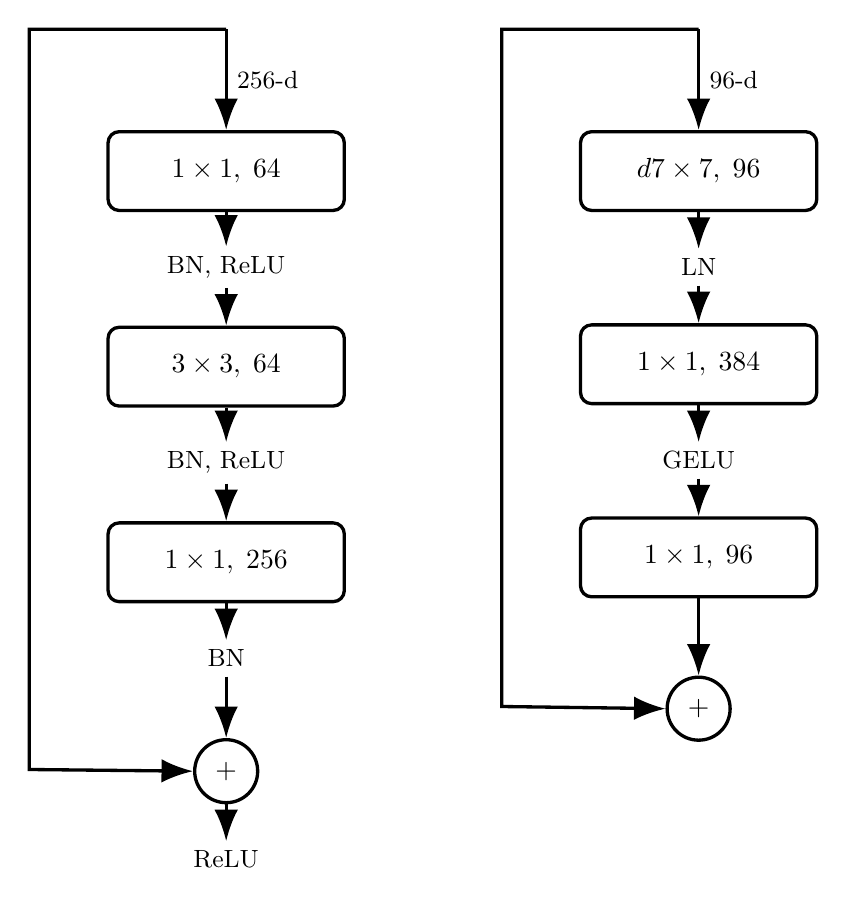
\begin{tikzpicture}[
  font=\sffamily,
  >={Latex[length=4mm,width=3mm]},
  line/.style={very thick, draw=black},
  box/.style={draw, very thick, rounded corners=4pt, align=center, minimum width=30mm, minimum height=10mm, fill=white},
  note/.style={align=center, font=\small},
  plus/.style={draw, very thick, circle, minimum size=8mm, inner sep=0pt, fill=white}
]

% =========================
% Left block (ResNet-like)
% =========================
\coordinate (Ltop) at (0,0);

\node[box] (L1) at ($(Ltop)+(0,-10mm)$) {$1\times1,\;64$};
\node[note] (Lbn1) at ($(L1.south)+(0,-7mm)$) {BN, ReLU};

\node[box] (L2) at ($(Lbn1.south)+(0,-10mm)$) {$3\times3,\;64$};
\node[note] (Lbn2) at ($(L2.south)+(0,-7mm)$) {BN, ReLU};

\node[box] (L3) at ($(Lbn2.south)+(0,-10mm)$) {$1\times1,\;256$};
\node[note] (Lbn3) at ($(L3.south)+(0,-7mm)$) {BN};

\node[plus] (Lplus) at ($(Lbn3.south)+(0,-12mm)$) {$+$};
\node[note] (Lrelu) at ($(Lplus.south)+(0,-7mm)$) {ReLU};

% main vertical arrows
\draw[line,->] ($(Ltop)+(0,8mm)$) -- node[right, font=\small] {256-d} (L1.north);
\draw[line,->] (L1.south) -- (Lbn1.north);
\draw[line,->] (Lbn1.south) -- (L2.north);
\draw[line,->] (L2.south) -- (Lbn2.north);
\draw[line,->] (Lbn2.south) -- (L3.north);
\draw[line,->] (L3.south) -- (Lbn3.north);
\draw[line,->] (Lbn3.south) -- (Lplus.north);
\draw[line,->] (Lplus.south) -- (Lrelu.north);

% skip connection (left loop)
\coordinate (Lin) at ($(Ltop)+(0,8mm)$);
\draw[line,->] (Lin) -- ++(-25mm,0) -- ++(0,-94mm) -- (Lplus.west);

% outer frame (left)
% \node[fit=(Lin) (Lrelu), draw, very thick, rounded corners=6pt, inner sep=8mm] (Lframe) {};

% =========================
% Right block (ConvNeXt/ViT-like)
% =========================
\coordinate (Rtop) at (60mm,0);

\node[box] (R1) at ($(Rtop)+(0,-10mm)$) {$d7\times7,\;96$};
\node[note] (Rln) at ($(R1.south)+(0,-7mm)$) {LN};

\node[box] (R2) at ($(Rln.south)+(0,-10mm)$) {$1\times1,\;384$};
\node[note] (Rgelu) at ($(R2.south)+(0,-7mm)$) {GELU};

\node[box] (R3) at ($(Rgelu.south)+(0,-10mm)$) {$1\times1,\;96$};
\node[plus] (Rplus) at ($(R3.south)+(0,-14mm)$) {$+$};

% main vertical arrows
\draw[line,->] ($(Rtop)+(0,8mm)$) -- node[right, font=\small] {96-d} (R1.north);
\draw[line,->] (R1.south) -- (Rln.north);
\draw[line,->] (Rln.south) -- (R2.north);
\draw[line,->] (R2.south) -- (Rgelu.north);
\draw[line,->] (Rgelu.south) -- (R3.north);
\draw[line,->] (R3.south) -- (Rplus.north);

% skip connection (right loop)
\coordinate (Rin) at ($(Rtop)+(0,8mm)$);
\draw[line,->] (Rin) -- ++(-25mm,0) -- ++(0,-86mm) -- (Rplus.west);

% outer frame (right)
% \node[fit=(Rin) (Rplus), draw, very thick, rounded corners=6pt, inner sep=8mm] (Rframe) {};

\end{tikzpicture}
\end{document}
